\bigskip

\item Which if the following is a graph for $y = \frac{1-x^2}{x-2}$.  (No calculators allowed.)

% \resizebox{5in}{!}{\includegraphics{SVC.01.06.110.ps}}
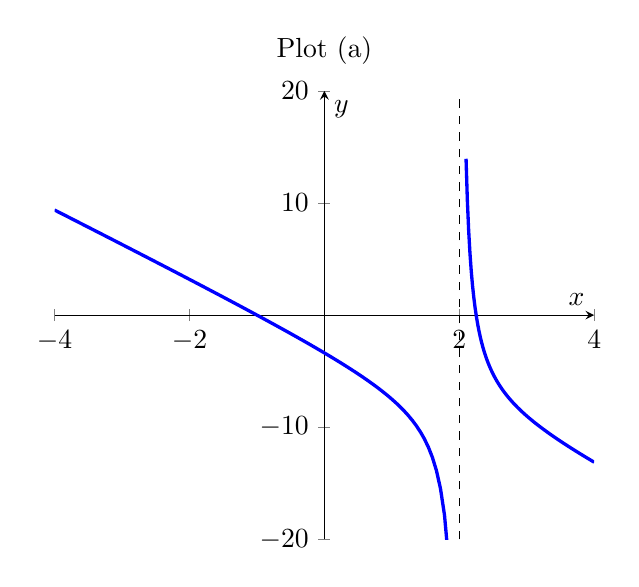
\begin{tikzpicture}
        \begin{axis}[axis lines=center, xlabel={$x$}, ylabel={$y$}, xmin=-4, xmax=4,
                ymin=-20, ymax=20, title={Plot (a)}]
                \addplot[color=blue, very thick, domain=-4:1.9, samples=100] {-3*(x+1)*(x-2.25)/(x-2)};
                \addplot[color=blue, very thick, domain=2.1:4, samples=100] {-3*(x+1)*(x-2.25)/(x-2)};
                \draw[dashed] (axis cs:2,-20) -- (axis cs:2,20);
            \end{axis}
        \end{tikzpicture}
    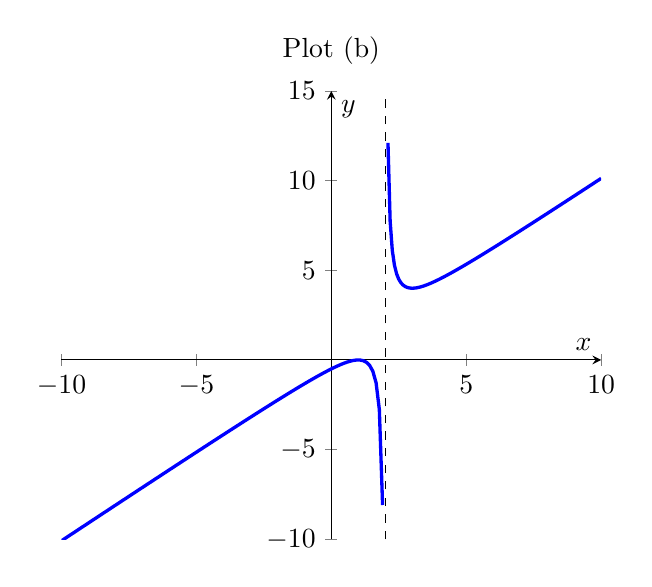
\begin{tikzpicture}
        \begin{axis}[axis lines=center, xlabel={$x$}, ylabel={$y$}, xmin=-10, xmax=10,
                ymin=-10, ymax=15, title={Plot (b)}]
                \addplot[color=blue, very thick, domain=-10:1.9, samples=100] {x+1/(x-2)};
                \addplot[color=blue, very thick, domain=2.1:10, samples=100] {x+1/(x-2)};
                \draw[dashed] (axis cs:2,-10) -- (axis cs:2,15);
            \end{axis}
        \end{tikzpicture}\\
    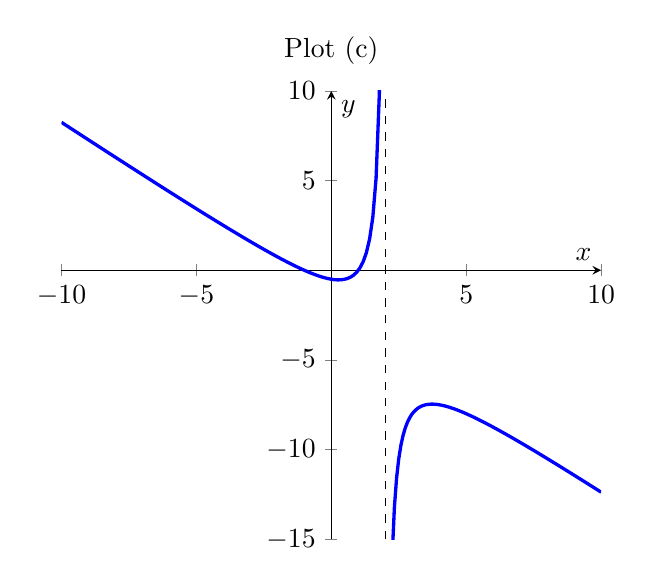
\begin{tikzpicture}
        \begin{axis}[axis lines=center, xlabel={$x$}, ylabel={$y$}, xmin=-10, xmax=10,
                ymin=-15, ymax=10, title={Plot (c)}]
                \addplot[color=blue, very thick, domain=-10:1.9, samples=100] {(1-x^2)/(x-2)};
                \addplot[color=blue, very thick, domain=2.1:10, samples=100] {(1-x^2)/(x-2)};
                \draw[dashed] (axis cs:2,-15) -- (axis cs:2,10);
            \end{axis}
        \end{tikzpicture}
    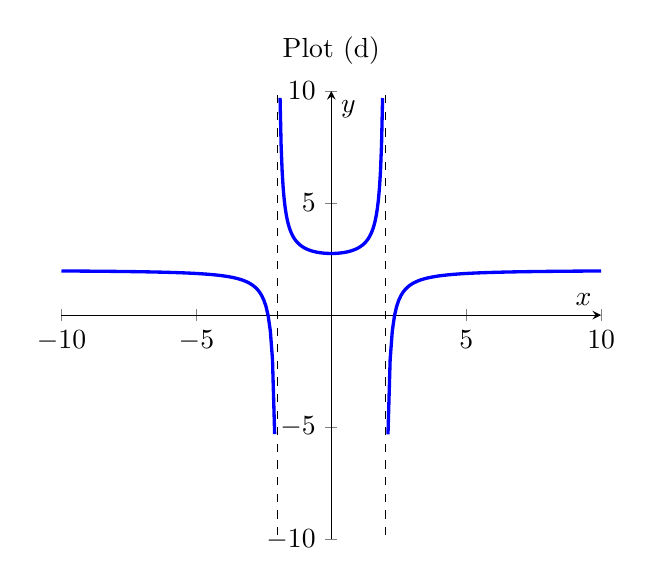
\begin{tikzpicture}
        \begin{axis}[axis lines=center, xlabel={$x$}, ylabel={$y$}, xmin=-10, xmax=10,
                ymin=-10, ymax=10, title={Plot (d)}]
                \addplot[color=blue, very thick, domain=-10:-2.1, samples=100]
                {(1-x^2)/((x+2)*(x-2))+3};
                \addplot[color=blue, very thick, domain=-1.9:1.9, samples=100]
                {(1-x^2)/((x+2)*(x-2))+3};
                \addplot[color=blue, very thick, domain=2.1:10, samples=100]
                {(1-x^2)/((x+2)*(x-2))+3};
                \draw[dashed] (axis cs:2,-15) -- (axis cs:2,10);
                \draw[dashed] (axis cs:-2,-15) -- (axis cs:-2,10);
            \end{axis}
        \end{tikzpicture}

% ConcepTests - to accompany Calculus 4th Edition, Hughes-Hallet et al. John Wiley \& Sons.
